\documentclass[11pt]{article}

\newcommand{\Moser}{M{\"o}ser}

\usepackage{algorithm2e}
\usepackage{amssymb}
\usepackage[english]{babel}
\usepackage{changepage}
\usepackage{cite}
\usepackage{float}
\usepackage[margin=1.5in]{geometry}
\usepackage{graphicx}
\usepackage{lmodern}
\usepackage{setspace}
\usepackage{tabularx}
\usepackage{url}

\usepackage[T1]{fontenc}

\bibliographystyle{acm}

\graphicspath{{figures}}

\onehalfspacing

\begin{document}
\thispagestyle{empty}
\begin{center}
\begin{Large}
\emph{Master's Thesis Proposal} \\
Department of Computer Science \\
Rochester Institute of Techology \\
\end{Large}
\vspace{4em}
{\huge Anonymity Analysis of Cryptocurrencies} \\
\vspace{3em}
{\LARGE Liam Morris} \\
{\tt lcm1115@rit.edu} \\
\vspace{3em}
\begin{adjustwidth}{.5in}{.5in}
Chair: Professor Stanis{\l}aw Radziszowski \hfill {\tt spr@cs.rit.edu} \\
\vspace{2em}
\hrulefill \\
\vspace{3em}
Reader: Professor Warren Carithers \hfill {\tt wrc@cs.rit.edu} \\
\vspace{2em}
\hrulefill \\
\vspace{3em}
Observer: Professor Bo Yuan \hfill {\tt bo.yuan@rit.edu} \\
\vspace{2em}
\hrulefill
\end{adjustwidth}
\vspace{2em}
Rochester, NY 14623 USA \\
\vspace{2em}
March 25, 2014
\end{center}
\pagebreak
\thispagestyle{empty}
\begin{abstract}
Cash in the real world allows for parties to exchange currency without the need
to go through some sort of central authority. One person, Alice, can simply hand
cash over to another person, Bob. In this transaction the only two people that
have knowledge of this exchange are Alice and Bob. Until recently there was no
electronic equivalent to this exchange. In 1982 David Chaum proposed a system of
anonymous electronic cash based on blind signatures, and in 1990 founded
DigiCash as an electronic cash company. There were a few banks that implemented
electronic cash systems, but these banks and DigiCash ultimately went bankrupt
in 1997 and 1998 despite the enthusiasm surrounding anonymous electronic cash.
Between 1998 and 2008 there were no successful implementations of electronic
cash that offer a decentralized, anonymous, and untraceable system.

In 2008 a paper was published by Satoshi Nakamoto on the cryptocurrency known as Bitcoin.
A cryptocurrency is a form of electronic cash backed by mathematical and
cryptographic constructs, unlike traditional currency which was historically
backed by gold or silver. Cryptocurrencies have seen rising popularity in recent
years due to their decentralized, distributed, peer-to-peer protocols. Part of
this rising popularity is also attributable to the supposed anonymity of these
protocols; however, due to the public transaction history required for these
protocols and the fact that transactions are pseudonymous and not purely
anonymous, this supposed anonymity may not exist. While the systems may achieve
the goal of decentralized currency it may not achieve the goal of
untraceability. In this thesis we will analyze the technical implementations
of Bitcoin and other cryptocurrencies to determine the level of anonymity
provided by these protocols. We will also research some proposed improvements 
to determine their feasibility.
\end{abstract}
\clearpage
\pagenumbering{arabic}
\tableofcontents
\listoffigures
\pagebreak
\section{Problem Statement}
Cash in the real world allows for parties to exchange currency without the need
to go through some sort of central authority. One person, Alice, can simply hand
cash over to another person, Bob. In this transaction the only two people that
have knowledge of this exchange are Alice and Bob. Until recently there was no
electronic equivalent to this exchange. In 1982 David Chaum proposed a system of
anonymous electronic cash based on blind signatures~\cite{chaum83}, and in 1990 founded
DigiCash as an electronic cash company. There were a few banks that implemented
electronic cash systems, but these banks and DigiCash ultimately went bankrupt
in 1997 and 1998 despite the enthusiasm surrounding anonymous electronic cash.
Between 1998 and 2008 there were no successful implementations of electronic
cash that offer a decentralized, anonymous, and untraceable system.

In 2008 a paper was published by Satoshi Nakamoto on the cryptocurrency known as Bitcoin~\cite{nakamoto08}.
A cryptocurrency is a form of electronic cash backed by mathematical and
cryptographic constructs, unlike traditional currency which was historically
backed by gold or silver. The Bitcoin protocol uses the SHA-256 algorithm as
part of its cryptographic foundation, while many others such as Litecoin are
founded on the scrypt key derivation scheme proposed by Colin Percival in
2009~\cite{percival09}.  Cryptocurrencies have seen rising popularity in recent
years due to their decentralized, distributed, peer-to-peer protocols. Part of
this rising popularity is also attributable to the supposed anonymity of these
protocols; however, due to the public transaction history required for these
protocols and the fact that transactions are pseudonymous and not purely
anonymous, this supposed anonymity may not exist. While the systems may achieve
the goal of decentralized currency it may not achieve the goal of
untraceability. There have been proposals in recent years such as the
Zerocoin~\cite{miers13} and Mixcoin~\cite{bonneau14} to remove all traceability
from the Bitcoin protocol. In this thesis we will analyze the technical
implementations of the Bitcoin and Litecoin protocols to determine the level of
anonymity and traceability provided by these protocols. We will research
proposed improvements, such as Zerocoin and Mixcoin, to determine their
feasibility and possible optimizations that can be made.

\section{Cryptographic Tools}

\subsection{Hash Functions}
A hash function is an algorithm that processes variable length inputs to produce
a fixed length digest. Hash functions are important for cryptocurrency protocols
as they provide the basis on which their proof-of-work schemes are constructed.

Cryptographic hash functions are designed in such a way that they are
non-invertible. In other words, if we have computed a digest of some message we
should not be able to easily deduce the message from the digest. For a hash
function to be secure, the following criteria must uphold~\cite{rogaway04}:

\begin{description}
    \item[Preimage Resistant] Given a digest $H(M)$, it must be computationally
        difficult to determine $M$.
    \item[Second Preimage Resistant] Given a message $M_1$, it must be
        computationally difficult to determine a second message $M_2$ such that
        $H(M_1) = H(M_2)$.
    \item[Collision Resistant] It must be computationally difficult to construct
        two messages $M_1$ and $M_2$ such that $H(M_1) = H(M_2)$.
\end{description}

Hash functions are frequently used to uniquely identify large messages so that
they may be efficiently signed. In the case of cryptocurrency protocols this
typically takes on the form of hashing an entire transaction so that just the
digest may be signed by a user. In a transaction between Alice and Bob, Alice
could construct a transaction and sign every parameter with her private
key individually, which must then be verified with her public key individually.
This amount of computation is wasteful on both ends, but Alice can use hashing to
reduce the amount of computation required. She can construct the transaction as
before, but instead of signing every component she can hash the transaction
parameters together and then sign the resulting digest. On the other end only
verification of the signed digest is required.

\subsubsection{Secure Hash Algorithm}
The Secure Hash Algorithm (SHA) is a family of algorithms published by the National
Institute of Standards and Technology (NIST). In order for an algorithm to be
included in the SHA family it must be selected as a winner by NIST in one of its
hash function competitions.

Bitcoin and Litecoin both use the SHA-256 variant of the SHA-2
algorithm as part of their proof-of-work scheme\footnote{Litecoin uses
{\sc scrypt} for its proof-of-work scheme, but {\sc scrypt} performs two
{\sc SHA-256} hashes as part of the algorithm.}. The SHA-256 function hashes a
message $M$ in the following manner~\cite{nist}:

\begin{enumerate}
    \item Pad $M$ so that it is on a 512-bit boundary.
    \item Divide $M$ into 512-bit blocks $M_1, M_2, \ldots, M_n$.
    \item Compute $H(M_i) = H(M_i) \boxplus H(M_{i - 1})$ for $i = 1$ to $n$,
        where $H(M)$ is defined as the hashing operation on one block,
        $H(M_0)$ is a fixed initial hash value, and
        $\boxplus$ is defined as integer addition modulo $2^{32}$.
    \item Output $H(M_n)$ as resulting hash.
\end{enumerate}

Currently NIST states that the SHA-2 algorithm is still cryptographically
secure\footnote{\url{http://csrc.nist.gov/groups/ST/hash/policy.html} --
Accessed 4-1-2014}. If a vulnerability is found then there is the potential for
attacks on cryptocurrencies, so it is worth examining the more recent SHA-3
Keccak family. The SHA-3 algorithm is not necessarily more secure than SHA-2;
however, it is very different structurally so it is unlikely that both SHA-2 and
SHA-3 would be vulnerable to a single attack.

The SHA-3 algorithm uses a
sponge construction, which processes variable length input to produce a
corresponding infinite length output. If a fixed length output
is desired the output of a sponge function is truncated to the specified
length. Given a permutation $f$, a sponge function operates in the following
manner~\cite{bertoni07}:
\vspace{1em}\\
\begin{algorithm}[H]
    \KwIn{$P$ = list of input characters, $n$ = desired hash length}
    \KwOut{$h_0, h_1, \ldots$ = output characters}
    $S \gets \emptyset$ \\
    \For{$p \in P$}{
        $S \gets f(S \oplus p)$
    }
    \For{$i = 1, 2, \ldots, n$}{
        {\sc Output($S$)} \\
        $S \gets f(S)$
    }
\end{algorithm}

\subsection{Elliptic Curve Digital Signature Algorithm Keys}
Bitcoin and Litecoin use the Elliptic Curve Digital Signature Algorithm (ECDSA)~\cite{johnson01}
as the basis for their public-private key system. Although the use of ECDSA
suggests that there is a central figure monitoring the public key
infrastructure, the specification for the ECDSA exists outside of the
cryptocurrency. The curve parameters for Bitcoin and Litecoin are specified by
{\tt secp256k1}\footnote{{\tt secp256k1} is used in the base
Bitcoin implementation located at \url{http://github.com/bitcoin} and in the base
Litecoin implementation at \url{http://github.com/litecoin-project}}\cite{secg}:
\vspace{1em}\\
\begin{tabularx}{\textwidth}{cX}
    $F_p$ & finite field where
        $p = 2^{256} - 2^{32} - 2^9 - 2^8 - 2^7 - 2^6 - 2^4 - 1$\\
    Curve $E$ & $y^2 = x^3 + ax + b$ over $F_p$ where\\
    & $a = 0$\\
    & $b = 7$\\
    Base $G$ & $G$ = 02 79BE667E F9DCBBAC 55A06295 CE870B07 029BFCDB 2DCE28D9
        59F2815B 16F81798 in compressed form\\
    & \\
             & $G$ = 04 79BE667E F9DCBBAC 55A06295 CE870B07 029BFCDB 2DCE28D9 59F2815B 16F81798 483ADA77 26A3C465 5DA4FBFC 0E1108A8 FD17B448 A6855419 9C47D08F FB10D4B8 in uncompressed form\\
    $Order(G)$ & $n$ = FFFFFFFF FFFFFFFF FFFFFFFF FFFFFFFE BAAEDCE6 AF48A03B
        BFD25E8C D0364141\\
    Cofactor $h$ & $h = 1$
\end{tabularx}

\subsection{Scrypt}
Scrypt is a password-based key derivation function developed by Colin Percival
in 2009~\cite{percival09}. Percival developed scrypt as part of the Tarsnap
backup service on UNIX-like systems in order to reduce the strength that
special purpose hardware provides to attackers when performing parallelized
brute force attacks on passwords. Scrypt plays an important role in
cryptocurrencies as it is the foundation on which Litecoin and its forks are
built~\cite{sprankel13}.

The methodology behind scrypt is that we can
reduce the effectiveness of parallelization by requiring the algorithm to have
enormous memory overhead. The reason for this memory overhead is that the
algorithm generates a large vector of pseudorandom strings which are then
accessed in pseudorandom order. The implication of this is that these strings
must be kept in memory to be accessed. In theory one could compute each string
as needed without storing the entire vector in memory, but the algorithm is
designed such that this computation is not trivial.

The structure of scrypt consists of the following elements:
\begin{description}
\item[ROMix] A method of pseudorandomly generating items and pseudorandomly
    accessing them.
\item[BlockMix] Transforms each block of input into a corresponding block of
    output using 1,024 rounds of the {\sc Salsa20/8} algorithm developed by Daniel
    Bernstein~\cite{bernstein08}.
\item[String Vector] The vector in which each block is stored throughout
    algorithm.
\end{description}

The overall process for deriving a key using scrypt is as follows:
\begin{enumerate}
    \item Compute initial hash using {\sc SHA-256}.
    \item Perform 1,024 rounds of \textbf{BlockMix} step using {\sc Salsa20/8}
        and record outputs in a vector.
    \item Perform 1,024 rounds of \textbf{BlockMix} again using {\sc Salsa20/8}
        with inputs chosen pseudorandomly (with output from previous iteration
        used to determine next block selection) from the vector and written
        pseudorandomly back to the vector.
    \item Hash resulting vector using {\sc SHA-256} again for collision
        resistance\footnote{{\sc Salsa20} does not provide collision resistance,
        so a separate step is needed to provide collision resistance.}.
    \item Output resulting hash.
\end{enumerate}

\section{Cryptocurrency Protocols}
Cryptocurrency protocols generally consist of three main components: a
transaction scheme, a verification scheme, and a transaction ledger. The specific
details for each of these may vary between protocols, but they typically exhibit
the same characteristics regardless of implementation. In particular, different
protocols may be constructed from different cryptographic primitives and tools,
as well as be set in entirely different mathematical domains.

\subsection{Bitcoin Protocol}
Bitcoin is the most widely used cryptocurrency and is the first cryptocurrency
to begin circulation. Many other cryptocurrencies are direct forks of Bitcoin,
so the Bitcoin protocol will be our primary focus.

\subsubsection{Transaction Scheme}
The transaction scheme of Bitcoin uses pseudonyms to specify a transaction
between users on the network. A transaction is recorded as a transfer of some
value from one user to another, where the input side of a transaction consists
of one or more public keys and the output side of a transaction consists of one
public key.
\vspace{1em}\\
\begin{minipage}{\linewidth}
The method of recording a new transaction of some bitcoin from Alice to Bob
is as follows:
\begin{enumerate}
    \item Alice signs the bitcoin's previous transaction signature with her
        private key
    \item The resulting value is used as an input in a hash function along
        with Bob's public key
    \item The output of this hash is the transaction signature, which can be
        signed with Bob's private key to initiate another transaction
\end{enumerate}
\end{minipage}
\vspace{1em}\\

Once a transaction has been created it is sent out to the Bitcoin network in
order to be verified, approved, and permanently recorded in the block chain.

\begin{figure}[H]
    \centering
    \caption[Bitcoin transaction process]{Bitcoin transaction process~\cite{nakamoto08}}
    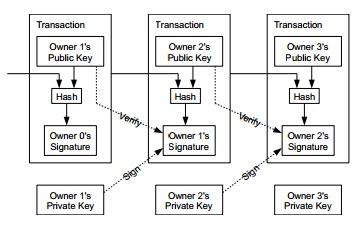
\includegraphics[width=.9\textwidth]{figures/transaction.png}
\end{figure}

\subsubsection{Verification Scheme}
Once a transaction has been initiated it must be verified by users in the
Bitcoin network in order for the transaction to be fully committed. Verification
of a transaction requires some proof-of-work in order to complete the block and
append it to the block chain. The proof-of-work scheme used by the Bitcoin
protocol is based on the Hashcash proof-of-work scheme proposed by Adam Back in
2002.~\cite{back02}. The original Hashcash specification was intended to prevent
denial of service attacks in email service but has found popular usage within
the Bitcoin protocol.
To complete proof-of-work for a transaction, a SHA-256 hash with inputs of the
previous hash and a nonce must be found such that the resulting hash is below a
specified difficulty level. In other words, we must feed the SHA-256 algorithm
the previous hash of the coin concatenated with a nonce or string such that we
have a specified number of leading 0's in the resulting hash. One common way of
computing proof-of-work is using the following algorithm:
\vspace{1em}\\
\begin{algorithm}[H]
    \KwIn{$D$ = difficulty parameter, $P$ = previous transaction hash}
    \KwOut{$N$ = nonce, $H$ = resulting hash}
    $N \gets 0$\\
    $H \gets ${\sc SHA-256({\sc Concat($P, N$)})}\\
    \While{H $\ge$ D}{
        $N \gets N + 1$\\
        $H \gets ${\sc SHA-256({\sc Concat($P, N$)})}
    }
    \Return{N, H}
\end{algorithm}\vspace{1em}

Once a proof-of-work has been determined the block with the proof-of-work
information is distributed to the Bitcoin network. The difficulty of the
proof-of-work operation is such that blocks are found for a transaction, globally 
on average, in 10 minutes. This time is based on the global block difficulty which
is determined by a ``moving average targeting an average number of blocks per
hour.''~\cite{nakamoto08} What this means is that periodically the speed at
which blocks are computed is evaluated and the global difficulty is adjusted
accordingly\footnote{Difficulty evaluation happens every 2016 blocks which is
specified by the {\tt bitcoind} client at \url{http://github.com/bitcoin}}.

The node which distributes the completed block to the network is rewarded with
bitcoins if the block is accepted. This reward starts out at 50 bitcoins per
block and is halved after every 210,000 blocks, which means that bitcoins
ultimately have an maximum quantity of roughly 21,000,000~\cite{nakamoto08}.

\subsubsection{Network Structure}
The original Bitcoin whitepaper~\cite{nakamoto08} describes the Bitcoin network in the following
way:
\begin{enumerate}
    \item Transactions are broadcast to all network nodes.
    \item Transactions are collected and joined to form a block.
    \item A proof-of-work for a block is found, which is then broadcast to all nodes.
    \item If the proof-of-work is valid, all transactions in a block are valid,
        and bitcoins involved have not already been spent, then the block is accepted.
    \item The accepted block is appended to the block chain, and its hash is now
        used as the input hash for the next block.
\end{enumerate}

In other words, all nodes in the network are made aware of new transactions,
verified transactions, and accepted blocks. In this way the transaction record
(block chain) is shared among all nodes in the network.

\subsection{Litecoin Protocol}
Litecoin is the second most widely used
cryptocurrency\footnote{\url{http://coinmarketcap.com} -- Accessed 3-18-14,
Litecoin has the second highest 24 hour trading volume}, and is itself a fork
of Bitcoin. Litecoin's first block was mined in October
2011\footnote{http://ltc.blockr.io/block/info/1}. Litecoin has a few key
differences from Bitcoin.
The primary difference between Litecoin and Bitcoin is how the coins
are mined, or rather how the transactions are verified. Rather than using
SHA-256 as a proof-of-work scheme Litecoin uses Colin Percival's 
scrypt~\cite{percival09}. Additionally, rather than a global average of 10
minutes per block as in Bitcoin, Litecoin targets a global average of 2.5
minutes~\cite{sprankel13}. To prevent the reward pool of litecoins from drying
up too quickly as a result of this faster verification time, the number of
blocks after which the reward is halved is
quadruple that of Bitcoin. Rather than halving after every 210,000 blocks, the
reward for verifying a block halves after every 840,000 blocks.

\subsubsection{Transaction Scheme}
The Litecoin transaction scheme is identical to that of
Bitcoin. Litecoin also records the signatures of all users involved, the amount
being transferred in a block which is then itself part of a larger block
chain.

\subsubsection{Verification Scheme}
Litecoin was forked from Bitcoin to address the strength that special purpose
hardware brings to Bitcoin. Users in the Bitcoin network with application
specific integrated circuits (ASIC) designed specifically for computing SHA-256
hashes have an enormous advantage over users without such hardware. To address
this Litecoin uses the scrypt~\cite{percival09} key derivation scheme instead of SHA-256,
which changes the hashing scheme from a CPU-bound operation to a memory-bound
operation. By changing the verification problem from a CPU-hard to memory-hard problem,
parallelization no longer improves the speed of solving the
problem. This yields the following Litecoin proof-of-work algorithm:
\begin{algorithm}
    \KwIn{$D$ = difficulty parameter, $P$ = previous transaction hash}
    \KwOut{$S$ = salt, $H$ = resulting hash}
    $S \gets 0$\\
    $H \gets ${\sc scrypt($P, S$)}\\
    \While{H $\ge$ D}{
        $S \gets S + 1$\\
        $H \gets ${\sc scrypt($P, S$)}\\
    }
    \Return{S, H}
\end{algorithm}

\subsubsection{Network Structure}
The network structure of Litecoin, much like the transaction scheme, is
virtually identical to that of Bitcoin. The network nodes are users connected to
the network who receive notifications of new transactions and verified
transactions.

\subsection{Current State of Anonymity}
Users in the Bitcoin community can be falsely led to the conclusion that their
transactions are purely anonymous. For example, WikiLeaks accepts bitcoin
donations and states\footnote{\url{http://shop.wikileaks.org/donate} --
Accessed: 3-25-14},
\begin{quote}
``Bitcoin is a secure and anonymous digital currency. Bitcoins cannot be easily
tracked back to you, and are safer and faster alternative to other donation
methods.''
\end{quote}
This quote was published in 2011 yet still remains as stated on the WikiLeaks
website as of March 2014 despite some criticism of its accuracy.

Each transaction contains identifying information with respect to the addresses
of the users. For every transaction in the block chain, we can see between which
users the transaction occurred as well as the number of bitcoins transferred.
Each of these transactions exists in the public transaction record to defend
against double spending of bitcoins. Due to the public nature of this record and
the information associated with each transaction it is possible to deduce some,
if not all, information about users on the network.

One way to deduce information about users is based on the input addresses into a
transaction. Since the private key owning a bitcoin is required to initiate a
transaction of that bitcoin, we can safely assume that in a transaction
with multiple input addresses that the addresses belong to one
entity or person. The other possible scenario is that private keys were shared,
but this is an unlikely scenario. In fact, in the original Bitcoin whitepaper,
Nakamoto states~\cite{nakamoto08},
\begin{quote}
``Some linking is still unavoidable with multi-input
transactions, which necessarily reveal that their inputs were owned by the same
owner.''
\end{quote}

Much research has been done in this area already. In 2011, Reid and Harrigan
analyzed one specific case of a theft of 25,000 BTC and attempted to trace the
stolen BTC through the Bitcoin network~\cite{reid11}. One of the important
results from this study was that it was not extraordinarily difficult to follow
the transfer of bitcoins between entities. The authors were able to successfully
trace the stolen bitcoins across many transfers and determine some specific
addresses to which the coins were transferred, such as LulzSec.

One way in which Nakamoto addresses this is suggesting that public keys be kept
anonymous; however, this is not ideal or even practical. Many users
publish their public keys in forum signatures so that they may receive bitcoins.
In this case, the public key is then very obviously associated with that
specific username and passive analysis of multi-input transactions can possibly
reveal other keys associated with that user. Even if users do not publish their
keys in this way, some association may be revealed if a user takes advantage of
services or stores that accept bitcoins. Consider the case of a user wanting to
exchange her bitcoins for some form of currency. To do so, she must go through
some Bitcoin exchange service, in which she necessarily reveals some personally
identifying information to be able to receive her money. She has now placed her
anonymity in the hands of the exchange, since if the exchange is compromised
her personal information is also compromised.

In 2013 Ron and Shamir~\cite{ron13} performed analysis on the Bitcoin network
using transaction size as their metric. First they performed similar analysis to
Reid and Harrigan to build a graph of entities, and then analyzed large
transactions to and from those entities. One of the first results from this
analysis is that they were able to easily identify a few key entities: Mt.
Gox\footnote{The largest bitcoin exhange at the time, filed for bankruptcy February 28,
2014l}, Instawallet\footnote{Another large bitcoin exhange, shut down April 3rd,
2013.}, and DeepBit\footnote{The largest mining pool at the time the study was
performed.}.

Another key result determined
from this analysis is the transaction patterns that are commonly used to attempt
to obscure a user's identity. The main activities identified by Ron and Shamir
are long chains, fork-merge patterns, and savings accounts. The long chains of
transactions begin as one or more large transactions which are then split into
many smaller transactions in a very long chain. Fork-merge patterns are similar,
except that the smaller transactions are eventually merged back into one
address. A large transaction gets split into multiple smaller transactions, but
all bitcoins ultimately end up back at the originating address. The last
activity observed was the use of Bitcoin ``savings accounts.'' Bitcoins are
distributed across many addresses after which they are essentially untouched. A
common pattern for all of these activities is splitting a transaction into equal
parts, which are then also split into equal parts, etc. The resulting structure
observed from this activity is akin to a tree~\cite{ron13}.

Researchers at University of California, San Diego and George Mason
University~\cite{meiklejohn13} performed analysis on change addresses in a
Bitcoin transaction. They used the assumption that a one-time
change address is controlled by the same user as the input addresses. Based on
this assumption, the authors were able to discover what they called ``peeling
chains,'' similar to activities observed by Ron and Shamir. This type of analysis
was applied to a rather peculiar Bitcoin wallet\footnote{Address: {\tt
1DkyBEKt5S2GDtv7aQw6rQepAvnsRyHoYM}}, in which an extremely large Bitcoin wallet
was split into several smaller wallets. These smaller wallets then eventually
interacted with some Bitcoin services, including exchanges. If this wallet were
associated with an entity such as the Silk Road or the Bitcoin Savings \& Trust
Ponzi scheme~\cite{moore13}, the exchanges might be inclined to reveal
identifying information about the user in question, ultimately eliminating any
notion of anonymity.

Using the result from these case studies we can clearly see that input addresses and
change addresses can be used to identify Bitcoin ``entities.'' We can also analyze
these entities more closely and see how the entities try to obscure their
identity. Since these sorts of patterns are not extraordinarily difficult to
deduce from the Bitcoin block chain, one can imagine a scenario where some law
enforcement agency might want to investigate a user who is a suspect in some
sort of illicit activity. We can determine a group of addresses that belong to
the user, and if any of those addresses interacted with a Bitcoin exchange or
service, the law enforcement agency could seize the personal
information of the user from such a service. Even further, we can see all
addresses with which the user interacted, which could implicate other users
involved in illicit activities. This allows the law enforcement agency to
closely analyze these users more closely, some of which may have interacted with
a Bitcoin exchange, and so on.

\subsection{Improving Anonymity}
There have been many attempts to resolve the anonymity issues present in the
Bitcoin protocol. Some of these attempts have arisen organically within the
Bitcoin community and are already in use, while others are proposed by academic
papers and have yet to be implemented.

\subsubsection{Mixer}
A very common form of obscuring one's identity is to use a mixer or
tumbler\footnote{This name comes from the devices used to clean physical coins.}.
These services are based on mix networks~\cite{chaum81}, which are used to mask
a user's identity within a network, such as the commonly used Tor network.
Unlike mix networks which are used to mix messages and anonymize the
users, Bitcoin mix services mix transactions to anonymize the users, frequently
charging some sort of processing fee for the service.

\begin{figure}[H]
    \caption[Example mix network]{Example mix network\protect\footnotemark}
    \centering
    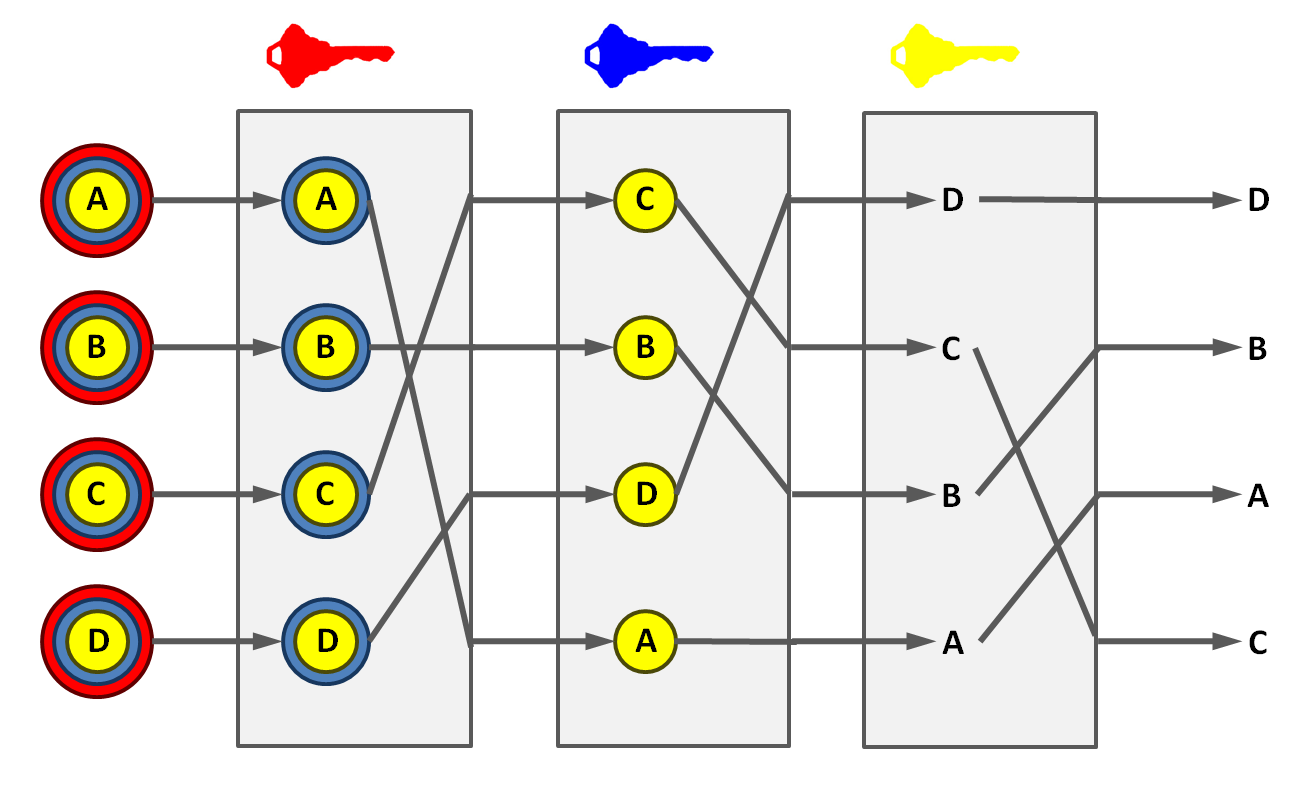
\includegraphics[width=.8\linewidth]{figures/mix.png}
\end{figure}

\footnotetext{\url{http://en.wikipedia.org/wiki/Mix_network} -- Accessed:
3-25-14}

A great deal of work has been done to analyze the anonymity provided by these services.
In 2013, Malte \Moser analyzed three popular mixing services: Blockchain.info,
Bitcoin Fog, and BitLaundry~\cite{moser13}. The key results of this experiment
were that Blockchain.info and Bitcoin Fog both used complex methods of
distributing transactions which eliminate the ability to discover any connection
between input and output transactions, effectively anonymizing the traffic.
BitLaundry, on the other hand, used direction connections between input and
output which allows for connections to be drawn across the mixing operations.
This imperfect anonymization is present in other mixers. In another study it
was observed that Bitcoin Laundry took input transactions and directly fed them
to output transactions effectively eliminating the purpose of the
service~\cite{meiklejohn13}. The possible cause for this is that the pool of
users in the service is to small to sufficiently anonymize transactions.

One of the primary issues in using these mixing or laundry services is that
trust must be placed in the service which is not an ideal scenario given that
one of the goals of Bitcoin is to eliminate the requirement to place trust in
individuals. It has even been observed that these services cannot necessarily be
trusted, as Meiklejohn reported that ``One of these, BitMix, simply
stole our money.''~\cite{meiklejohn13} The presence of this behavior and the
desire for anonymity suggests that there is a desire for a system which provides
anonymity without the need to place trust in some sort of central figure.

\subsubsection{Zerocoin}
In 2013, researchers at Johns Hopkins University proposed an extension to
improve Bitcoin's anonymity known as Zerocoin~\cite{miers13}. The group claims
that Zerocoin ``uses standard cryptographic assumptions and does not introduce
new trusted parties or otherwise change the security model of Bitcoin.'' The
basic idea is to add newly minted coins to an accumulator and then with the
assistance of zero-knowledge proofs spend the coins from the accumulator without
revealing a user's identity.

The Zerocoin protocol essentially creates a currency within Bitcoin. To mint
zerocoins, a user adds his bitcoins to the Zerocoin accumulator and receives
serial numbers in return, which correspond to the zerocoins that were ``minted.''
To later redeem the coins, the user must initiate a ``Zerocoin Spend'' transaction
and specify an output Bitcoin address. Upon verification of the bitcoins'
presence in the accumulator by a zero-knowledge proof the
corresponding bitcoin value is sent to the specified output address.

\begin{figure}[H]
    \centering
    \caption[Bitcoin block chain (a) and Zerocoin block chain (b)]{Bitcoin block
        chain (a) and Zerocoin block chain (b)~\cite{miers13}}
    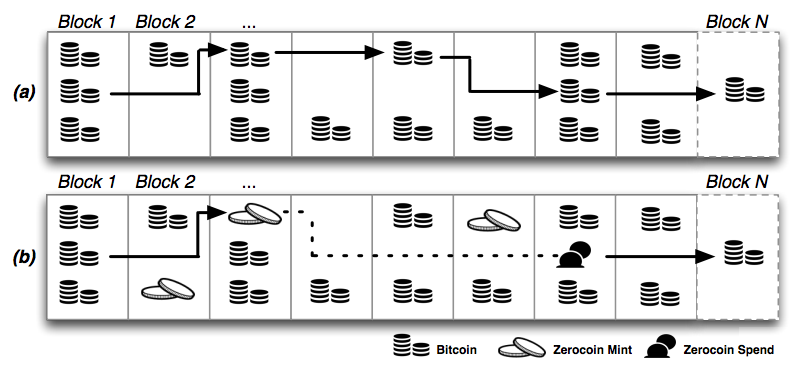
\includegraphics[width=\linewidth]{figures/zerocoin.png}
\end{figure}

This system creates anonymity by pooling all users' bitcoins together, and then
allowing for redemption of a random set of bitcoins from the pool, as long as
the user can prove that the bitcoins exist in the pool. In a sense, this is
analogous to a mixing service, but there is no requirement to place trust in any
figure, as the system is provably secure under certain cryptographic
assumptions.

\subsubsection{Mixcoin}
In 2014, another extension to improve anonymity in current Bitcoin protocol
was proposed under the name of Mixcoin~\cite{bonneau14}. This protocol
describes a method of establishing mixing services with some concept of
warranty, rather than modifying the Bitcoin protocol itself.

In general, sufficiently large mixing services do an acceptable job at providing
anonymity to users; however, these services have an inherent risk in that users
must entrust the service with their bitcoins in order to utilize the service.
If a mixing service steals a user's bitcoins, there is no way to prove that the
theft occurred. Mixcoin's goal is to address this issue by proposing a
construction for a mixing service that has built-in accountability.

The basic process behind Mixcoin is that before any mixing occurs, a user Alice
contacts the mix service and declares the following
parameters~\cite{bonneau14}:\\
\begin{tabular}{cl}
    $v$ & the value (chunk size) to be mixed\\
    $t_1$ & the deadline by which Alice must send funds to the mix\\
    $t_2$ & the deadline by which the mix must return funds to Alice\\
    $\kappa_{out}$ & the address where Alice wishes to transfer her funds\\
    $\rho$ & the mixing fee rate Alice will pay\\
    $n$ & a nonce, used to pay randomized mixing fees\\
    $w$ & the number of blocks the mix requires to confirm Alice's payment
\end{tabular}\vspace{1em}\\
Once the mix accepts the terms of the mix, a new escrow address $\kappa_{esc}$
is generated. All parameters plus $\kappa_{esc}$ are returned to Alice, signed
by the mixing service. This allows Alice to publicly claim with certainty that
the mixing service has stolen her funds in the event of theft, or in the case
that the funds have not been delivered to $\kappa_{out}$ by $t_2$.

While Mixcoin resolves one of the issues with mixing services it does not solve
every issue. The mixing service still effectively behaves as a bank between
users, which violates the goal of decentralized electronic cash. Additionally,
Mixcoin states that all records of a mix occurring should be deleted once the
mix is completed. If a mixer fails to do so and becomes compromised then the
information of all users that have utilized the service is also compromised.
Even though Mixcoin makes it easier for Alice to trust a mixer with her service,
she still needs to trust the service with her information. This means that even
if Mixcoin is utilized that there still may be some degree of traceability in
the system.

\section{Proposed Work}
The first part of research will consist of continued analysis of existing
work on cryptocurrency anonymity as well as existing proposals to address
cryptocurrency anonymity. It is clear that a great deal of attention has already
been directed towards the anonymity of the Bitcoin protocol, but similar
research and analysis has not been performed on other cryptocurrencies, such as
Litecoin.

We will investigate anonymity concerns of other cryptocurrency protocols and
determine if there are parallels with the Bitcoin community. If this is the
case, we will see what attempts (if any) have been made to address privacy
issues, as well as see if proposals to anonymize Bitcoin can be applied these
cryptocurrencies. Additionally, research that has been performed on the Bitcoin
transaction graph, such as identifying entities based on transaction inputs,
will be performed on the transaction graphs of other cryptocurrencies.

After researching current implementations and proposals it is important to
determine their feasibility. Indeed, one of the main goals of this thesis is to
analyze the computational overhead required to add anonymity to
cryptocurrencies. This may require implementing these protocols through software
if no public software implementations exist. Once we have an implementation of
these systems we will conduct performance benchmarking to determine the
computational complexity present in the protocols.

The ideal outcome of this work would be that one or more of these systems can be
implemented with minimal computational cost. In the case that the base
systems are not computationally feasible, we will perform more in-depth research
into possible improvements that can be made to specific algorithms to improve
performance while maintaining the same overall functionality. It is possible
that such changes could be significant enough to warrant a formal writeup of a
new protocol, but this would be a welcome side-effect and not one of our
primary goals.

\section{Deliverables}
Upon completion of all proposed work a thesis report will be submitted.
Contained in this thesis will be all background research, experiment results,
and any other required documentation. Additionally, the following software will
be submitted:
\begin{itemize}
    \item Libraries for any cryptocurrency extensions that are implemented,
    \item Library for performing benchmarks on cryptocurrency systems.
\end{itemize}

\section{Timeline}
The writing of the thesis, software implementation, and research will all be
done in parallel. A proposed schedule is as follows:
\begin{center}
\begin{tabularx}{\textwidth}{X|X}
    Date & Task\\
    \hline
    April 25, 2014 & Complete thesis proposal submission\\
    May 16, 2014 & Perform block chain analysis on Litecoin\\
    May 27 2014 -- August 22 2014 & \emph{Summer co-op}\footnote{Research will
                                    continue, but there is no formal timeline for
                                    this period of time. There will still be a
                                    progress email and website update every two
                                    weeks.}\\
    September 5, 2014 & Finish required background research, begin software
                        implementation\\
    September 19, 2014 & Finish software implementation, begin benchmarking and
                         recording data\\
    October 3, 2014 & Complete data analysis, revisit software implementation
                      for optimizations\\
    October 17, 2014 & Benchmark optimizations and record changes\\
    November 14, 2014 & Finish thesis report\\
    December 12, 2014 & Defend thesis\\
\end{tabularx}
\end{center}

\bibliography{references}

\end{document}
